\scanpage{27}
Soit $f$ comme dans Cor. 2, \inserted{mais on suppose $f$ un épi. effectif.} On veut prouver que $f$ est un morphisme de descente \uline{effective}. Soit donc $A'$ schéma abélien sur $S'$, avec donnée de descente relativement à $S'\mathbin{-}S$; prouver que cette donnée est effective.

a) Réduction au cas $S$ local \inserted{$=\operatorname{Spec}R$}: \uline{triviale}, par passage à la limite.
\deleted{\unsure{On y procède par récurrence sur} \illegible{3}, \unsure{sachant que le cas} \illegible{1} \unsure{est effectif dans le cas formel des schémas affines}.}

b) Réduction au cas $S$ local complet: \unsure{coup usuel} Alg. des.

Grâce au critère de descente plate des schémas abéliens de Raynaud. Mais il faut savoir que $S'_2\mathbin{-}S_2$ est \inserted{morphisme} de descente pour la catégorie des schémas abéliens relatifs, et on ne peut directement appliquer le \deleted{lemme 1, car} cor. 2, car $S_2$ n'est plus loc. noeth! Mais on s'en tire en remarquant qu'il est vrai \deleted{\unsure{que l'on}} ici que (avec les notations de la dém. du lemme 1)
\diagram{\begin{tikzcd}[ampersand replacement=\&,column sep=small,row sep=small]
S\arrow[r,dash]\arrow[d,dash]\&S'\arrow[r,equal]\arrow[d,dash]\&S''\arrow[r,equal]\arrow[r,dash]\&S'''\&\text{1-descente}\\
S_1\arrow[r,dash]\arrow[d,equal]\&S'_1\arrow[r,equal]\arrow[d,equal]\&S''_1\arrow[r,equal]\arrow[r,dash]\arrow[d,equal]\&S'''_1\arrow[d,equal]\&\text{1-descente}\\
S_2\arrow[r,dash,"f_2"']\arrow[d,equal]\arrow[d,dash]\&S'_2\arrow[r,equal]\arrow[d,equal]\arrow[d,dash]\&S''_2\arrow[r,equal]\arrow[r,dash]\arrow[d,equal]\arrow[d,dash]\&S'''_2\arrow[d,equal]\arrow[d,dash]\&\text{1-descente}\\
S_3\arrow[r,dash]\&S'_3\arrow[r,equal]\&S''_3\arrow[r,equal]\arrow[r,dash]\&S'''_3\&\text{0-descente}
\end{tikzcd}}
\deleted{$A$ est radiciel sur \unsure{\text{$h_2$}} $f_2$}
\[
\operatorname{Ker}(f_{2*}O_{S'_2}\rightrightarrows h_{2*}(O_{S''_2}))
\]
est radiciel sur $\underline O_{S_2}$, car tout provient par chgt de base plat de la situation
\[
O_S\longrightarrow\operatorname{Ker}(f_*(O_{S'})\rightrightarrows h_*(O_{S''})).
\]
\margin{\figure{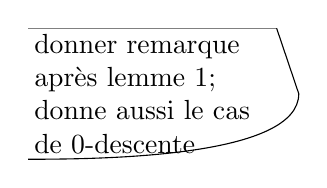
\begin{tikzpicture}\node[align=left,text width=3cm,inner sep=2pt](m){donner remarque après lemme 1; donne aussi le \unsure{cas de} 0-descente};\draw[gray] (m.north west) .. controls +(2,0) .. (m.north east);\draw (m.north east) -- ([xshift=8pt]m.east) .. controls +(0,-.8) and +(1,0) .. (m.south west);\end{tikzpicture}}}

\deleted{c) \deleted{\unsure{Cas à 2 étages}} Cas \deleted{$\unsure{S}$ dim $S=0$.} \inserted{$S$ réduit dim $S=0$ (et \unsure{le corps résiduel alg. clos})} On se ramène au cas où $S'$ est fini sur $S$ (quitte à prendre un sous-schéma fini \deleted{\unsure{de $S'$}} assez gros de $S'$), puis par \uline{factorisation}, se ramener au cas où $\operatorname{long}_A A'/A=1$. Alors le critère de descente par plate \unsure{est vérifié}: \unsure{trouver des} ouverts affines recouvrant $A'$, stables par \deleted{\unsure{des}} données de descente. Or pour ça, on est ramené au cas où $A$ est le spectre d'un corps, où c'est trivial.
\margin{\deleted{expliciter du point de vue \unsure{``carré de descente''}}}

d) Construction d'un schéma formel \inserted{abélien} sur $\operatorname{Spf}R$, qui descend le schéma formel défini par $A'$ (complété suivant la fibre de $A'_s$\unsure{\ldots}). \deleted{\unsure{Immédiat}} \inserted{Facile} \unsure{preuve}).}
\mspage{26}
